% Математические методы: операции с экспертным оценками (сложение, усреднение, сравнение)

\label{sec:math_methods_global}

Для анализа экспертных оценок надо определить математические объекты, как выступающие непосредственно в роли моделей экспертных оценок, так и вспомогательные, и определить допустимые математические операции над ними. 

Как уже говорилось, в качестве модели экспертной оценки числа $x \in X \subset \R$ можно взять разные математические объекты: % (см.  \ref{sec:intro_subjective})
\begin{enumerate}
  \item Одно число из того же множества $X$: $\hat{x} \in X$. Такую модель назовём точечной экспертной оценкой, или оценкой первого типа;
  \item Пара действительных чисел $a_1,\, a_2 \in X$, задающая интервал $[a_1,\, a_2]$. Такую модель назовём интервальной экспертной оценкой, или оценкой второго типа;
  \item Заданная таблицей, графиком или иным образом функция $p(\cdot)$, определённая на заданном множестве $X$, принимающая значения на отрезке $\zo$, см. рисунок \ref{ris:fuzzy_number_intro}.  Подобный объект, благодаря работам \cite{citeZadeh, dubois_prade-1990}, часто называют нечётким числом, поэтому назовём такую модель нечёткой экспертной оценкой (или оценкой третьего типа). В вырожденном случае, если только для одной точки $x_0 \in X$ упомянутая функция отлична от нуля, можно говорить о <<чётком>> или <<дельтообразном>> виде нечёткой оценки.
\end{enumerate}

Операции над точечными экспертными оценками идентичны операциям над значениями оцениваемого параметра  $x \in X$  в той шкале, в которой последние интерпретируются лицом, принимающим решение, и чаще всего их можно считать заданными в количественной шкале (как цена единицы товара или как оценки в школе) \cite{Mirkin}. Такие оценки можно сравнивать, пользуясь естественной упорядоченностью числовой прямой. Для таких оценок, полученных от разных экспертов, чаще всего можно вычислять среднюю оценку, характеризующую коллективное мнение экспертов. 

\subsection{Интервальные экспертные оценки}

В рамках точечной экспертной оценки эксперт не может выразить неуверенность, частичное или полное незнание, возможность нескольких сценариев развития исследуемого объекта. Простейшее для эксперта решение этих проблем --- задавать оценку в виде двух чисел вместо одного.

\subsubsection{Интервальная математика}

Интервальная математика упоминается c 1966 года в работах Мура~\cite{moore1966interval, moore2009introduction}. Она была разработана, в первую очередь, как база для моделирования неопределённости данных физических измерений при обработке этих данных на ЭВМ. Данным физических измерений присущи погрешности как случайного, так и неслучайного (систематического) характера, и интервальные числа не привязаны к конкретной модели их формирования. Поэтому они подходят и для моделирования неопределённости, присущей экспертным оценкам, если эксперт испытывает и высказывает неуверенность. 

Интервальные экспертные оценки следует рассматривать как заданную экспертом пару не случайных чисел $a_1 \leq a_2 \in X$, между которыми, по его мнению, заключён оцениваемый параметр $x \in X$, не известный эксперту на момент выставления оценки.  Интервалы со случайными границами, в т.\,ч. доверительные интервалы, в настоящей работе не рассматриваются.

Сравнение интервалов $A = [a_1,\,a_2]$ и $B = [b_1,\,b_2]$ можно осуществлять, например, таким образом:
\begin{equation*}
    A > B \Leftrightarrow b_1 > a_2. 
\end{equation*}
Сложение двух интервалов  определяется у Мура как покоординатное сложение: $A + B = [a_1+b_1,\,a_2+b_2]$. Среднее арифметическое двух интервалов, заданных разными экспертами, можно считать коллективным мнением экспертов, как и в случае точечных экспертных оценок.

С другой стороны, можно рассмотреть интервальные оценки как подмножества числовой прямой, на множестве которых можно ввести отношение частичного порядка. Эту идею мы частично позаимствовали у Феллера \cite{cit:feller}.

\subsubsection{Частичный порядок интервалов}
\label{order_int}

Отношение частичного порядка <<$\prec$>> заключается, по определению, в следующем:
\begin{equation}
\label{interv_order}
\begin{split}
\forall A: & A \prec A; \\
\forall A, B: & A \prec B \text{ и } B \prec A \Rightarrow A = B; \\
\forall A, B, C: & A \prec B \text{ и } B \prec C \Rightarrow A \prec C.
\end{split}
\end{equation}

Конструктивно, для интервалов $A, B$:  $A \prec B$ тогда и только тогда, когда $A \subset B$. Порядок частичный, поскольку существуют не вложенные друг в друга интервалы. Однако, для любых двух интервалов $A, B$ можно ввести бинарную операцию, сопоставляющую им такое множество $C$, что $C \succ A$ и $C \succ B$, причём всякое другое $C' \neq C: C' \succ A, C' \succ B$ будет содержать в себе $C$. Это есть определение точной верхней грани множества всех интервалов, которые включают в себя $A$ и $B$:
\begin{equation}
\label{interv_sup}
 C = A \vee B.
\end{equation}
Часто, для краткости, выражение \eqref{interv_sup} произносят как <<супремум  $A$ и $B$>>. Конструктивно, супремум двух интервалов --- это их объединение $A \cup B$. Аналогично вводится инфинум $A$ и $B$, обозначаемый $A \wedge B$ и конструктивно эквивалентный их пересечению $A \cap B$.

Операции <<$\vee$>> и <<$\wedge$>> содержат глубокий физический смысл: они позволяют найти коллективное экспертное мнение в модели интервальных оценок, не противоречащее мнению отдельно взятых экспертов. Так, если $A, B$ --- мнения двух экспертов, то $A \vee B$ отражает доверие со стороны лица, принимающего решение и к тому, и к другому эксперту, т.е. это лицо допускает и варианты развития событий, предсказанные как первым, так и вторым экспертом. Инфинум  $A \wedge B$ отражает, напротив, недоверие к экспертам, оставляя лишь общую часть заданных ими интервалов в качестве коллективного мнения.

\subsection{Нечёткие экспертные оценки и теории возможностей}

В случае использования интервальных экспертных оценок эксперт не указывает {\sl предпочтительность} тех или иных значений $x \in [a_1,\, a_2]$. Если же она указана, получается оценка третьего типа --- нечёткая экспертная оценка. Эти более сложные оценки могут моделироваться с помощью упомянутых в разделе~\ref{sec:intro_decision} теорий нечётких множеств и теории возможностей.
%\cite{citeZadeh, dempster, tahani, dubois_prade-1990}

\todo[inline]{Необходимо чётко разделить разные теории возможностей: теорию возможностей Заде и её аналоги, теорию возможностей Пытьева. В первой есть аксиомы, но нет шкалы значений возможности. У Пытьева есть шкала, но нет аксиом. }

С момента своего появления в 70-х годах прошлого века, теории возможностей изначально предназначены для моделирования неопределённости субъективного характера, связанной с принципиальной невозможностью точного определения множества исследуемых объектов (например, множества высоких людей) или с неполнотой знаний об исследуемом объекте, выраженных экспертными оценками. Это принципиально отличает данные теории от теории вероятностей, несмотря на внешнюю схожесть математических аппаратов этих теорий. 

Возможность (или возможностная мера) в теории возможностей Заде~\cite{citeZadeh} и её аналогах (далее просто <<теория Заде>>) можно определить аналогично тому, как в теории вероятностей определяется вероятность~\cite{dubois_prade-1990}. Пусть $\Omega$~--- множество элементарных событий, и $\Po(\Omega)$~--- $\sigma$-алгебра всех подмножеств множества $\Omega$, тогда 
\label{def_possibility}
возможностью называется всякая функция $\P:\ \Po(\Omega)\to[0,1]$, удовлетворяющая следующим аксиомам:
\begin{compactenum}
\item $\P(\varnothing) = 0$,\label{axiom_P1}
\item $\P(\Omega) = 1$,\label{axiom_P2}
\item $\P\Big(\bigcup\limits_{A\in\Alg} A\Big) = \sup\limits_{A\in\Alg}\P(A)$, для любого множества событий $\Alg\subset\Po(\Omega)$.\label{axiom_P3}
\end{compactenum}

Аксиомы возможности (в теории Заде) аналогичны аксиомам вероятности~\cite{kolmogorov}, но алгебраические операции над значениями возможности~--- другие. Вместо обычного сложения в теории возможностей используется операция <<$\max$>> (в случае бесконечного числа слагаемых~--- <<$\sup$>>), а вместо умножения --- операция <<$\min$>> (в бесконечном случае~--- <<$\inf$>>):
\begin{equation}
\label{operations_zadeh}
    a \plus b = \max\{a,\, b\}, \quad a \mult b = \min\{a,\, b\}, \quad a,\,b \in [0,1].
\end{equation}
%sad... Говорят, что значения возможности заданы в шкале $\scL = \scale$: они лежат на отрезке $\zo$, могут сравниваться как действительные числа, и присутствуют бинарные операции <<$\plus$>> и <<$\mult$>>, в качестве которых используются <<$\max$>> и <<$\min$>> соответственно. 
Эти операции не выводятся, а постулируются в рамках теории возможностей Заде, однако в них есть определённый <<здравый смысл>>, который можно пояснить на примере. \label{example_zadeh}
\begin{example}
Пусть множество элементарных событий есть множество дверей различной ширины, $\Om = \setN$ -- их индексы. В замкнутой комнате есть двери, составляющие некоторое подмножество $A \subset \setN$ (заранее неизвестно, какие именно).  Эксперимент заключается в том, что надо войти в комнату и пронести через двери широкий предмет, но неизвестно, пролезет он, или нет. 

Если двери расположены в комнате параллельно (можно пройти через любую из них), то возможность пронести предмет определяется шириной двери, имеющей максимальную ширину из имеющихся дверей. Если же двери расположены последовательно (длинная анфилада комнаток), то возможность пронести предмет определятся минимальной шириной двери из тех, что будут на пути.
\todo[inline]{Или про биологический принцип (не помню, как называется), согласно которому биологическая система в каждый момент времени реагирует на наиболее сильный раздражитель.}
\end{example}

\begin{notice}
Выше изложен аксиоматический подход, развиваемый Дюбуа и Прадом~\cite{dubois_prade-1990}. Изначально же теория возможностей Заде основана на его теории нечётких множеств \cite{ZadehPrime}. В теории нечётких множеств в первую очередь формулируются свойства некой функции принадлежности $\mu_{F}(\cdot): X \rightarrow \zo$, где $\mu_F(x)$ --- степень принадлежности числа $x \in X$ нечёткому множеству $F$. 

Пусть нечёткое множество $F$ с функцией принадлежности $\mu_{F}$ является нечётким ограничением \cite{citeZadeh} оцениваемого параметра, моделируемого числом $x \in X$. Например, $x$ --- возраст человека, $F$ --- утверждение <<этот человек --- молодой>>, а $\mu_{F}(x)$ интерпретируется как <<степень соответствия>> возраста $x \in X$ утверждению $F$. Тогда по определению полагается $\P(\cdot) \defeq \mu_{F}(\cdot)$. В нашем примере это означает, что возможность того, что возраст человека окажется равным $x$, если эксперт утверждает, что <<человек молодой>>, численно равна <<степени соответствия>> этого возраста нечёткому множеству <<молодость>>. 
\todo[inline]{Если есть аксиомы возможности, то с них всё и начинается, и не нужны никакие нечёткие множества. Если же хочется связать теорию возможностей с теорией нечётких множеств, то тогда постулируются свойства функций принадлежности, а из них вытекают постулаты возможностной меры. Нужно это указать, чтобы не было путаницы.}
\end{notice}
\begin{notice}
Вместо равенства $\Pr(A) + \Pr(\Omega\setminus A) = 1$, устанавливающего однозначную связь между вероятностью всякого события $A\in\Po(\Omega)$ и его отрицанием, в теории возможностей получаем
\begin{equation}
\label{max_PA_PnotA}
    \max\{\P(A), \P(\Omega\setminus A)\} = 1.
\end{equation}
Равенство~\eqref{max_PA_PnotA} интерпретируется как факт, состоящий в том, что из двух противоположных событий по крайней мере одно безусловно возможно. В то же время оно не определяет однозначной связи между $\P(A)$ и $\P(\Omega\setminus A)$, что согласуется со стремлением при моделировании субъективных суждений не устанавливать жёсткой связи между показателями, свидетельствующими в пользу некоторого события, и показателями, свидетельствующими против него~\cite{dubois_prade-1990}.
\end{notice}

\label{zadeh_fuzzy_asset_alg}
В качестве модели нечёткой оценки возможность Заде можно использовать следующим образом. Возьмём некий интервал $X$ в качестве множества элементарных событий, на которых эксперт задаёт функцию $p(\cdot): X \rightarrow [0,1]$, причём он обязательно выбирает точку $x_0$, для которой $p(x_0) = 1$. Тогда этой функции можно однозначно сопоставить возможность $\P(\{x\}) \define= p(x) \in \zo,\; x\in X$ с введёнными для значений возможности алгебраическими операциями \eqref{operations_zadeh}. 

В частности, эксперт может задать функцию $p$ лишь на интервале $A \subset X$ (причём в самом тривиальном случае он может положить $p(x) = 1\; \forall\, x \in A$, что сводит оценку к интервальному типу). Тогда функцию $p$ следует продолжить вне этого интервала на $X$ значениями $p(x) = 0\, \forall\; x \notin A$. Множество $A$ становится носителем $p$, а также носителем порождаемой этой функцией возможностной меры $\P$. Носитель $p$ обозначается символом $\supp\; p$.

Существуют, однако, фундаментальные проблемы в рамках теории возможностей Заде и её аналогов:
\begin{enumerate}
\item
Операции сложения (<<$\max$>>) и умножения (<<$\min$>>) значений возможности звучат логично (см. пример на странице \pageref{example_zadeh}), но ниоткуда не выводятся.
\item
Не прослеживается связь теории возможностей, призванной моделировать субъективные суждения, и математической статистики, призванной моделировать случившиеся факты, хотя эта связь должна быть установлена, когда факты имеются в наличии.
\item
В теории возможности Заде и её аналогах содержательно интерпретируются конкретные числовые значения возможности. Проблема тут вот в чём.
Когда эксперт выставляет оценку $\hat{x}  \in X$ (первого типа) в виде балла, например, $X = \{1, 2, ..., 10\}$, существует специальный регламент относительно того, какой смысл несёт каждый балл $x \in X$. Каждый случай проведения экспертизы требует разработки регламента и установления соглашения между экспертами. Этот процесс постоянно совершенствуется, но до сих пор в таких регламентах остаётся немало неопределённости. Представим теперь, что необходимо договориться не только по поводу смысла значений $x \in X$, но и по поводу смысла значений $\p(\cdot) \in \zo$, что требуется для сохранения содержательной интерпретации каждого конкретного числа отрезка $\zo$ всеми экспертами одновременно. Это создаст неподъёмную нагрузку на экспертов и разработчиков экспертизы и является главным недостатком теории возможностей Заде. 
\end{enumerate}
Эти недостатки устранены в рамках теории возможностей Ю.~П.~Пытьева.

\subsection{Теория возможностей Ю.~П.~Пытьева как средство моделирования нечётких экспертных оценок}
\label{sec:math_methods_ours}

В конце 1990-ых~--- начале 2000-ых профессором Московского университета Ю.\,П.\;Пытьевым предложен новый вариант теории возможностей~\cite{possbook, cit:smf, probbook, pytyev_experts}. Этот вариант принципиально отличается от теории возможностей Заде и её аналогов наличием принципа относительности возможности, который требует инвариантности любых выводов, полученных в рамках теории, относительно группы монотонно возрастающих непрерывных преобразований $\gamma(\cdot):\ [0,1]\to[0,1]$, $\gamma(0) = 0,\ \gamma(1) = 1$ значений возможности. При моделировании экспертных оценок данный принцип позволяет каждому эксперту задавать значения возможностей в своей собственной субъективной шкале, заботясь лишь о правильной (с точки зрения эксперта) упорядоченности возможностей событий.

\subsubsection{Происхождение теории возможностей Ю.~П.~Пытьева. Шкала значений возможности}

В отличие от теории возможностей Заде и её аналогов, теория возможностей Пытьева изначально разработана как альтернатива теории вероятностей при моделировании стохастической случайности.  В этом качестве, возможность всякого события $A$, определённого на $\sigma$-алгебре $\Po(\Omega)$ из вероятностного пространства $\OAPr$, должна служить мерой его относительной (относительно других событий) <<предопределённости>>. Возможность события $A$ обозначим $\P(A)$, пока не определяя, что такое есть возмонжностная мера $\P$ в теории Пытьева. 
\begin{notice}
Ю.\,П.\;Пытьевым показано~\cite{possbook2}, что одна и та же возможностная модель позволяет моделировать стохастический эксперимент, вероятностная модель которого может изменяться от испытания к испытанию.  Им дана частотная интерпретация возможности, состоящая в том, что в достаточно длинной серии независимых испытаний частота более возможного события почти наверное больше частоты менее возможного. 
\end{notice}

Из этих соображений значения возможности,  как и значения вероятности, моделируются числами из отрезка $\zo$. Их можно сравнивать, пользуясь естественной упорядоченностью числовой прямой <<$\leqs$>>, и к ним применяется теоретико-вероятностная нормировка:
\begin{enumerate}
\item\label{item_poss_rel_1}
    $\P(\varnothing) = \Pr(\varnothing) = 0$.
\item\label{item_poss_rel_2}
    $\P(\Omega) = \Pr(\Omega) = 1$.
\end{enumerate}

Конструкция $\scL = \scale$ называется шкалой значений возможности, где в качестве бинарных алгебраических операций <<$\plus$>> и <<$\mult$>>  со значениями возможностей используются <<$\max$>> и <<$\min$>> соответственно вместо обычных операций сложения и умножения из теории вероятностей. Эти операции \emph{выводятся} из принципа относительности возможности.

\subsubsection{Принцип относительности возможности}
\label{sec:sec_20151029_02}

Обозначим $\bTheta$ множество всех строго монотонных непрерывных функций ${\gamma(\cdot):\ [0,1]\to[0,1]}$, таких что $\gamma(0) = 0$, $\gamma(1) = 1$. Множество $\bTheta$ есть группа относительно операции композиции <<$\circ$>>: $\forall\;\gamma_1, \gamma_2 \in \bTheta: \gamma_1 \circ \gamma_2 \in \bTheta$.

Как известно, отношение <<$\leqs$>> в шкале $\scL$ значений возможности, введённое выше как естественное отношение порядка действительных чисел, обладает следующим свойством:
\begin{equation}
\label{eq:20151115_01}
    \text{если } a \leqs b, \text{ то } \gamma(a) \leqs \gamma(b)
\end{equation}
для любых ${a,\, b\in\scL},\ {\gamma(\cdot)\in\bTheta}$. С учётом того, что на возможность $\P$  не налагается никаких требований, кроме условий \ref{item_poss_rel_1})--\ref{item_poss_rel_2}), приведённых выше, свойство~\eqref{eq:20151115_01} приводит к следующему принципу (относительности возможности), занимающему центральное место в теории возможностей Ю.\,П.\;Пытьева:
\begin{center} \fbox{ 
\begin{minipage}{0.9 \textwidth}
Возможности $\P$ и $\P'$ эквивалентны, если найдётся такая функция $\gamma(\cdot)\in\bTheta$, что $\P'(A) = \gamma(\P(A)),\ {A\in\Po(\Om)}$, а утверждения и выводы, сформулированные в рамках возможностной модели, определяемой возможностью $\P$, содержательны, если и только если они остаются верными при замене $\P(\cdot)$ на $\P'(\cdot) = \gamma(\P(\cdot))$ для любой функции ${\gamma(\cdot)\in\bTheta}$.
\end{minipage}
} \end{center}

\begin{comment}
Обозначим $\bTheta$ множество всех монотонно возрастающих непрерывных функций $\gamma(\cdot):\ [0,1]\to[0,1]$, таких что $\gamma(0) = 0$, $\gamma(1) = 1$. Согласно \emph{принципу относительности} возможности $\P$ и $\P'$ считаются эквивалентными, если найдётся такая функция $\gamma(\cdot)\in\bTheta$, что $\P(A) = \gamma(\P'(A)),\ A\in\Alg$, а утверждения и выводы, сформулированные в рамках возможностной модели, определяемой возможностью $\P$, считаются содержательными, если и только если они остаются верными при замене $\P(\cdot)$ на $\P'(\cdot) = \gamma(\P(\cdot))$ для любой функции $\gamma(\cdot)\in\bTheta$.
\end{comment}

Поясним сформулированный принцип на примере двух утверждений:
\begin{itemize}
\item
    <<Возможность $\P(A)$ события $A$ равна $0.9$>>.\\
    Данное утверждение в теории возможностей не является содержательным, так как найдётся такая функция $\gamma(\cdot)\in\bTheta$, что величина $\gamma(\P(A))=\gamma(0.9)$ не будет равна $0.9$.

\item
    <<Возможность события $A$ больше, чем возможность события $B$ (событие $A$ более возможно, чем $B$)>>.\\
    Такое утверждение, в отличие от предыдущего, может быть содержательно истолковано, так как для любой функции $\gamma(\cdot)\in\bTheta$ из соотношения $\P(A)>\P(B)$ следует $\gamma(\P(A))>\gamma(\P(B))$.
\end{itemize}

Эти примеры демонстрируют характерную особенность теории возможностей, являющуюся прямым следствием принципа относительности: никакие значения возможностей кроме $0$ и $1$ не являются информативными, содержательно может быть истолкована лишь упорядоченность возможностей событий. Этот факт позволяет задать возможность $\P$ в возможностной модели стохастического эксперимента исходя лишь из представления о том, какие события являются более возможными, а какие~--- менее возможными.

\subsubsection{Алгебраические операции в шкале значений возможности. Возможностная мера}
\label{sec:sec_20151029_03}

В~\cite{possbook, possbook2} доказана следующая теорема.
\begin{theorem}
\label{th:plus_mult_operations}
Если бинарные операции $\plus$ и $\mult$ являются коммутативными непрерывными отображениями $[0,1]\times[0,1]\to[0,1]$, и для любых $a,\, b\in[0,1]$, $\gamma(\cdot)\in\bTheta$
\begin{gather*}
    a\plus b = b\plus a, \quad a\mult b = b\mult a,\\
    0\plus a = a, \quad 0\mult a = 0, \quad 1\plus a = 1, \quad 1\mult a = a,\\
    \gamma(a\plus b) = \gamma(a) \plus \gamma(b); \quad \gamma(a\mult b) = \gamma(a) \mult \gamma(b),
\end{gather*}
то операции $\plus$ и $\mult$ суть
\begin{equation}
\label{20151029_01}
    a \plus b = \max\{a,\, b\}, \quad a \mult b = \min\{a,\, b\}, \quad a,\,b \in [0,1].
\end{equation}
\end{theorem}

Ещё раз подчеркнем, что, в отличие от возможности в теории Заде, значения возможности Пытьева заданы в ранговой шкале. Теорема \ref{th:plus_mult_operations} даёт ответ на вопрос, как \emph{должны} быть, в силу принципа относительности возможностей, определены алгебраические операции над \emph{числовыми} значениями возможностей в такой шкале, если никакие значения возможности, кроме неподвижных относительно группы $\bTheta$ точек $0$\footnote{Равенство $\P(\{\om\}) = 0$ означает принципиальную невозможность элементарного события $\om$.} и $1$, не являются информативными, и содержательно может быть истолкована лишь их упорядоченность. Поэтому теорема \ref{th:plus_mult_operations} позволяет определить шкалу $\scL=\scale$ как отрезок $[0,1]$ с естественной упорядоченностью действительных чисел и алгебраическими операциями~\eqref{20151029_01}.

\emph{Возможностью} (или возможностной мерой) $\P$ называется функцией, определённая на $\sigma$-алгебре $\Po(\Omega)$ подмножеств множества элементарных событий $\Omega$ и принимающей значения в шкале $\scL=\scale$:
\begin{equation*}
    \P:\ \Po(\Omega)\to\scL.
\end{equation*}
Заметим, что в отличие от вероятности возможность $\P$ всегда может быть определена на алгебре \emph{всех} подмножеств $\Omega$, в связи с чем в дальнейшем всегда будем считать $\Po(\Omega) = 2^\Omega$. В теории возможностей всякое множество $A\in\Po(\Omega)$ называется событием, а тройка $\OAP$ называется пространством с возможностью или возможностным пространством. 

\subsubsection{Нечёткий элемент и нечёткая экспертная оценка}

В теории возможностей Пытьева предусмотрена формальная конструкция, облегчающая использование теории для моделирования нечёткой экспертной оценки, алгоритм которого, в простейшем случае, идентичен приведённому на странице \pageref{zadeh_fuzzy_asset_alg} алгоритму для возможности Заде. Речь идёт о понятии нечёткого элемента.

Будем считать, что определено некоторое пространство элементарных событий $\Om$, из которых в наблюдении истинного значения параметра, осуществимого только \emph{после} проведения экспертизы, реализуется только одно. Функция
\begin{equation*}
	\tilde x(\cdot): \Om \rightarrow X,
\end{equation*} 
сопоставляющая каждому элементарному событию значение $x \in X$, называется нечётким элементом.  

Например, пусть эксперт оценивает параметр, значение которого, неизвестное на момент выставления оценки, обозначим по-прежнему $x \in X$. В силу неопределённости (см. раздел \ref{sec:intro_uncertainty}) в знаниях эксперта, с точки зрения последнего в роли \emph{самого} параметра (а не его значения) выступает как раз нечёткий элемент $\tilde x$.

Нечёткий элемент в теории возможностей полностью задаётся своим распределением $\p^{\tilde x}(\cdot): X \rightarrow \zo$, сопоставляющим каждому его значению возможность этого значения. Такое распределение при моделировании субъективных суждений задаётся субъектом (экспертом) и является, таким образом, нечёткой экспертной оценкой $p(\cdot) = \p^{\tilde x}(\cdot)$. Разумеется, оно порождает возможностную меру, поскольку $\p^{\tilde x}(x)$ есть ни что иное, как возможность события $\{\tilde x(\om) = x\}, \om \in \Om, x \in X$.

Считается, что, аналогично случайной величине в теории вероятностей, нечёткий элемент из <<полного>> пространства с возможностью $\OAP$ порождает через своё распределение $\p^{\tilde x}$ <<урезанное>> пространство с возможностью $(X, \Po(X), \P^{\tilde x})$, где $\Po(X)$~--- множество всех подмножеств $X$, и
\begin{equation*}
	\P^{\tilde x}(A) = \sup_{x \in A} \p^{\tilde x}(x), A \in \Po(X).
\end{equation*} 
В некотором частном случае для простоты можно считать, что пространство элементарных событий (математически моделируемое \emph{числовым множеством}) совпадает с множеством $X$. В таком случае меры $\P^{\tilde x}$ и $\P$ совпадают, что и приводит нас к алгоритму моделирования нечётких оценок на странице \pageref{zadeh_fuzzy_asset_alg}.

Используя такую модель экспертной оценки, можно предоставить эксперту свободу выбора своей субъективной шкалы, и экспертные оценки на рис. \ref{ris:fuzzy_ass03} будут выражать одно и то же экспертное мнение.
\begin{figure}[h]
\center{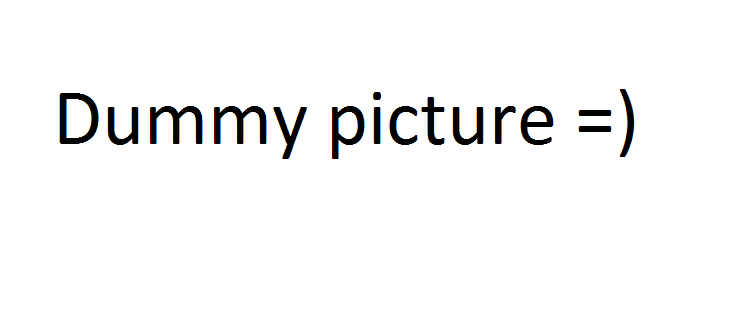
\includegraphics[width=0.7\linewidth]{./pic/dummy}}
\caption{\small Пример двух эквивалентных нечётких экспертных оценок.}
\label{ris:fuzzy_ass03}
\end{figure}

В рамках настоящей работы идея с введением отношения порядка, изложенная в разделе~\ref{order_int} для интервальных оценок, была развита и реализована применительно к нечётким оценкам как распределениям нечёткого элемента в теории возможностей Пытьева, что позволило использовать технику вычисления верхних и нижних граней для нахождения оценки, выражающей коллективное мнение экспертов,не противоречащее мнениям отдельных экспертов. См. раздел~\ref{preorder_pyt}.

